

\documentclass[10pt,twocolumn]{article}

% use the oxycomps style file
\usepackage{oxycomps}

% usage: \fixme[comments describing issue]{text to be fixed}
% define \fixme as not doing anything special
\newcommand{\fixme}[2][]{#2}
% overwrite it so it shows up as red
\renewcommand{\fixme}[2][]{\textcolor{red}{#2}}
% overwrite it again so related text shows as footnotes
%\renewcommand{\fixme}[2][]{\textcolor{red}{#2\footnote{#1}}}

% read references.bib for the bibtex data
\bibliography{references}

% include metadata in the generated pdf file
\pdfinfo{
    /Title (Predicting Solar Radiation using Machine Learning Techniques )
    /Author (Julia Chun)
}

% set the title and author information
\title{Comprehensive Project: {Solar Radiation Prediction Using Machine Learning}}
\author{Julia Chun}
\affiliation{Occidental College}
\email{jchun2@oxy.edu}

\begin{document}

\maketitle

\section{Problem Statement }
Climate change and global warming are global concerns where the implications are crucial and urgent. Changes to Earth's climate are driven by increased human emissions of greenhouse gases and these effects are seen having widespread effects on the environment. This concern is not a future problem as it was reported that effects that had long predicted would result from global climate change are now occurring, such as sea ice loss, accelerated sea level rise, and longer, more intense heat waves. Furthermore, these environmental implications impact various sectors of society and are interrelated. For instance, factors such as drought and flooding not only could cause damages to ecosystems and infrastructure, but could also impact food production and human health. In addition, these implications would exacerbate socio-economic inequalities as affected areas with less resources will be more vulnerable. Human activity will ultimately determine the severity of the effects caused by climate change and with any further delay in global action to reduce the causes of climate change, a future of a habitable environment could be missed.

Solar radiation prediction plays a critical role in optimizing renewable energy systems and advancing climate science. This project focuses on predicting Global Horizontal Irradiance (GHI) using machine learning techniques, leveraging data from the National Solar Radiation Database (NSRDB).  Global Horizontal Irradiance (GHI) is a critical measure in solar energy applications, representing the total solar radiation received on a horizontal surface at a given location. Accurate prediction of GHI is essential for optimizing solar energy systems, enhancing energy efficiency, and supporting the integration of renewable energy into the grid. However, modeling GHI is challenging due to the complex interplay of atmospheric conditions, geographic factors, and temporal variations.

This paper explores and compares different machine learning techniques—linear regression, decision trees, and stacking regressors—for modeling and predicting GHI at a given location. The primary goal is to assess the effectiveness of each technique in capturing the intricate patterns of solar radiation and providing reliable predictions.

.

Solar energy systems require accurate radiation forecasts to optimize their efficiency. Challenges could be faced regarding limitations in handling non-linear relationships and dynamic environmental factors. The implications of this project could extend to environmental sustainability and economic efficiency, showcasing its broader significance in combating climate change and advancing green technologies.

\section{Technical Background}

\subsection{Key Solar Radiation Indicators in the Dataset}

The dataset utilized for this study contains several key solar radiation indicators that are fundamental to understanding and modeling solar energy systems. These indicators are essential for assessing the availability and variability of solar energy at a given location and are widely used in renewable energy research. Below is an explanation of the primary solar radiation indicators included in the dataset:

\subsubsection{Global Horizontal Irradiance (GHI)}
\begin{itemize}
     GHI represents the total solar radiation received per unit area on a horizontal surface. It is the sum of Direct Normal Irradiance (DNI) and Diffuse Horizontal Irradiance (DHI), adjusted for the angle of incidence of the sun.GHI is the most commonly used metric for photovoltaic (PV) systems, as it captures both direct and diffuse solar radiation. It provides a comprehensive measure of the total energy available for solar power generation on flat or slightly tilted surfaces. This feature could be usedin the design, performance assessment, and optimization of PV systems. It is also crucial for energy forecasting and resource assessment.
\end{itemize}

\subsubsection{Direct Normal Irradiance (DNI)}
\begin{itemize}
     DNI measures the amount of solar radiation received per unit area on a surface that is always perpendicular (normal) to the sun's rays. DNI accounts for only the direct beam of sunlight, excluding scattered or reflected radiation. It is highly sensitive to clear sky conditions and obstructions such as clouds or shading. This measure could be critical for concentrating solar power (CSP) systems, which rely exclusively on direct sunlight to generate energy. DNI is also used to calculate GHI and assess solar resource potential.
\end{itemize}

\subsubsection{Diffuse Horizontal Irradiance (DHI)}
\begin{itemize}
    DHI quantifies the portion of solar radiation that is scattered by the atmosphere and reaches the Earth's surface from all directions. It excludes the direct beam of sunlight. DHI becomes particularly important in cloudy or overcast conditions, where the contribution of direct sunlight is minimal. It reflects the impact of atmospheric conditions on solar radiation. This feature could be useful for designing systems in regions with high cloud cover or for understanding the contribution of diffuse light to overall energy generation.
\end{itemize}

\subsubsection{Global Normal Irradiance (GNI)}
\begin{itemize}
     GNI measures the total solar radiation received on a surface that is perpendicular to the sun’s rays. It is similar to DNI but includes the diffuse component when the surface is oriented directly toward the sun. GNI is useful for assessing the potential solar energy capture of surfaces that track the sun throughout the day. This feature can be relevant for solar tracking systems and for calculating energy yield in systems designed to maximize direct sunlight capture.
\end{itemize}

\subsubsection{Relationship Between Indicators}

These indicators are interrelated and together provide a complete picture of solar radiation at a given location:
\begin{itemize}
    \item \textbf{GHI} is calculated as:
    \[
    GHI = DNI \cdot \cos(\theta) + DHI
    \]
    where \( \theta \) is the solar zenith angle (the angle between the sun's rays and the vertical axis).
    \item \textbf{DNI} and \textbf{DHI} are independent components that reflect different aspects of solar radiation—direct and scattered light, respectively.
    \item \textbf{GNI} complements these by considering the orientation of the receiving surface relative to the sun.
\end{itemize}

\subsubsection{Importance in Solar Energy Applications}

Understanding and utilizing these indicators can be essential for applications such as determining the suitability of different solar technologies (e.g., PV systems, CSP systems) for a given location or evaluating the energy yield and efficiency of solar installations under varying conditions. Furthermore, this could be useful when predicting solar energy availability to optimize grid integration and resource allocation.
\end{itemize}

\subsection{Machine Learning Models Used}

The project utilizes three machine learning models: linear regression, decision tree regression, and stacking regression. These models were chosen to explore the predictive capabilities of both simple and complex techniques for handling the relationships within the solar radiation dataset. Below is an explanation of each model:

\subsubsection{Linear Regression}
     Linear regression is a fundamental machine learning technique that models the relationship between a dependent variable (e.g., GHI) and one or more independent variables (e.g., temperature, cloud type) as a linear equation. The strength of a linear regression model is how it is interpretable, computationally efficient, and works well for features with strong linear relationships to the target variable. However, there are limitaions of a linear regression model as it struggles with capturing nonlinear relationships, which are common in solar radiation data due to factors like atmospheric scattering and cloud cover.


\subsubsection{Decision Tree Regression}
A decision tree regression is a non-linear model that splits the dataset into subsets based on feature values, forming a tree structure. Each split aims to minimize the variance within the resulting subsets. Decision trees can capture complex, nonlinear relationships and interactions between features. They are also interpretable, as the splits provide insight into the importance of features. Decision trees are prone to overfitting, especially with deep trees or when noise is present in the data.
\end{itemize}

\subsubsection{Stacking Regression}
A stacking regression is an ensemble learning technique that combines the predictions of multiple models (e.g., linear regression and decision tree) to produce a final prediction. The combined model, or meta-model, learns how to weight the contributions of the base models.Stacking can capture both linear and nonlinear relationships by leveraging the complementary strengths of different models. It often achieves higher accuracy than individual models. However, stacking could introduces additional computational complexity and may overfit if not properly tuned.
\end{itemize}

\subsubsection{Comparison and Rationale for Selection}
\begin{itemize}
    \item \textbf{Linear Regression:} Selected for its simplicity and interpretability, serving as a baseline for comparison with more complex models.
    \item \textbf{Decision Tree Regression:} Included for its ability to handle nonlinear dependencies and provide insights into feature importance.
    \item \textbf{Stacking Regression:} Chosen for its capacity to integrate multiple models, addressing both linear and nonlinear patterns for enhanced predictive performance.
\end{itemize}

By employing these models, the study aims to assess the effectiveness of different machine learning approaches in predicting solar radiation, offering insights into their strengths, limitations, and applicability to renewable energy systems.


\section{Literature Review}

Accurate prediction of solar radiation, particularly Global Horizontal Irradiance (GHI), is critical for optimizing solar energy systems and supporting the integration of renewable energy into the grid. Several machine learning (ML) techniques, including linear regression, decision trees, and stacking regressors, have been explored to enhance predictive accuracy. Additionally, the selection of relevant features and the target variable plays a pivotal role in improving model performance. This section reviews relevant research, discusses the implications of feature and target variable selection, and highlights how these studies influenced the direction of this project.

\subsection{Linear Regression, Decision Trees, and Stacking Regressors in Solar Radiation Prediction}
Linear regression, being a simple and interpretable model, serves as a baseline for predictive tasks. However, it is limited to capturing linear relationships. Decision trees, on the other hand, can model complex, nonlinear interactions and hierarchical patterns in the data. Combining these models using stacking regressors has shown promise in leveraging the strengths of both techniques. Stacking regressors use a meta-learner, often linear regression, to aggregate predictions from base models, thereby improving accuracy and robustness.

Kumari and Toshniwal \cite{14} evaluated linear regression, decision trees, and other ML techniques for GHI prediction across 21 cities in India. Their results demonstrated that decision trees and ensemble models significantly outperformed linear regression, particularly for datasets exhibiting nonlinear patterns. Furthermore, random forest, a closely related ensemble technique, consistently provided higher predictive accuracy, emphasizing the potential of combining multiple models for solar radiation prediction. This inspired the inclusion of stacking regressors in this project, combining the simplicity of linear regression with the robustness of decision trees to achieve better predictions.

\subsection{Feature Selection and Its Importance}
Feature selection is a critical step in building accurate and efficient models. Including irrelevant or redundant features can lead to overfitting, increased computational complexity, and reduced interpretability. Studies like 'Effect of Feature Selection on the Prediction of
Direct Normal Irradiance' \cite{4} highlight the importance of selecting impactful features such as GHI, Direct Normal Irradiance (DNI), and Diffuse Horizontal Irradiance (DHI). By using tree-based models like random forest and XGBoost to assess feature importance, they demonstrated that focusing on key predictors enhances both prediction accuracy and computational efficiency.

This project was influenced by these findings to prioritize feature selection. The use of feature importance rankings from decision trees ensured that only the most relevant meteorological and temporal features were included, optimizing both model performance and interpretability.

\subsection{Target Variable: Global Horizontal Irradiance (GHI)}
GHI is the most commonly used target variable in solar radiation prediction due to its direct relevance to solar energy applications. Representing the total solar radiation received on a horizontal surface, GHI serves as a key input for designing and optimizing photovoltaic systems. Accurate GHI prediction is essential for estimating solar energy potential, improving energy efficiency, and supporting grid integration of solar power.

The paper 'Global Horizontal Irradiance' \cite{8}, emphasize that GHI prediction benefits from ensemble models that leverage diverse features and data sources. GHI's dependence on meteorological and temporal variables necessitates incorporating these factors into predictive models to capture its inherent variability. This insight guided the focus on GHI as the primary target variable in this project, ensuring alignment with real-world solar energy applications.

\subsection{Key Takeaways}
\begin{itemize}
    \item \textbf{Model Exploration:} Linear regression serves as a baseline but struggles with complex patterns. Decision trees effectively capture nonlinear relationships, while stacking regressors combine the strengths of multiple models to achieve higher accuracy.
    \item \textbf{Feature Selection:} Selecting relevant features, such as temperature, humidity, pressure, and temporal variables, is crucial for improving model performance and reducing computational overhead. Tree-based methods provide robust feature importance metrics.
    \item \textbf{Target Variable Selection:} GHI is the preferred target variable due to its applicability in solar energy projects. Accurate prediction of GHI supports efficient design and operation of solar systems.
\end{itemize}

By leveraging linear regression, decision trees, and stacking regressors, along with robust feature and target variable selection techniques, this study aims to advance the field of solar radiation modeling. These approaches ensure accurate, interpretable, and computationally efficient predictions of GHI, facilitating the development of sustainable energy solutions. Insights from the literature not only guided the choice of models but also informed the importance of feature selection and the use of GHI as the target variable, ensuring the project's alignment with best practices in solar radiation prediction.

\bibliographystyle{unsrt}
\bibliography{references}



\section{Methods}

The methodology involved data collection, target variable selection, data preprocessing, feature selection, model selection, model training, and evaluation to systematically analyze and predict Global Horizontal Irradiance (GHI) using various modeling techniques . 

\subsection{Data Acquisition} 
\subsubsection{Database}
The datasets utilized for this study was sourced from the National Solar Radiation Database (NSRDB), a comprehensive dataset maintained by the National Renewable Energy Laboratory (NREL). The NSRDB is a trusted resource that provides high-resolution solar radiation data, offering information critical for solar energy research, system design, and performance assessment. The dataset is freely available and has been widely used in renewable energy projects and academic research.
\subsubsection{Dataset content}
The datasets collected for this study were specifically extracted for predefined geographic locations based on given latitude and longitude coordinates. All the datasets studied included the same features. For each location (specific latitude and longitude), data was retrieved for a specified year, ensuring temporal consistency in the analysis. Each dataset includes 27 distinct features, encompassing meteorological,atmospheric, solar radiation features, cloud-related, and temporal features. Examples of some features included in the dataset include solar radiation metrics such as Global Horizontal Irradiance (GHI), Direct Normal Irradiance (DNI), and Diffuse Horizontal Irradiance (DHI), as well as additional parameters like air temperature, relative humidity, wind speed, atmospheric pressure, and cloud cover. Temporal features such as hour, day, and month provide further granularity.
This alignment with prior work ensures the datasets contain all critical variables influencing solar radiation, facilitating robust predictive modeling and meaningful comparisons with established methodologies. The resulting data forms a foundation for the analysis, reflecting diversity and ensuring compatibility with proven solar energy modeling practices.



\subsection{Target Variable Selection}
The target variable selection process involved determining Global Horizontal Irradiance (GHI) as the primary variable for prediction, compared to other solar radiation metrics such as Direct Normal Irradiance (DNI), Diffuse Horizontal Irradiance (DHI), and Global Normal Irradiance (GNI). This decision was based on both practical relevance and the scope of this study. Furthermore, this variable seemed to most frequently studied as the target variable in other works. Because this variable represents the total amount of solar radiation received on a horizontal surface and combines both DNI (direct sunlight) and DHI (diffuse radiation scattered by the atmosphere), it makes the most comprehensive and practical measure for photovoltaic (PV) systems, which typically operate on flat or slightly tilted surfaces.  GHI’s practicality, versatility, and relevance to solar energy applications make it the most appropriate target variable for this study, offering significant advantages over other solar radiation indicators.
\subsection{Feature Exploration}

The initial step in the methodology involved exploring the relationships between features and the target variable, \textit{Global Horizontal Irradiance (GHI)}. This feature exploration was conducted using scatter plots, correlation heatmaps, and other visualizations to gain insights into the nature of these relationships and inform subsequent model selection.

\subsubsection{Linear Relationships}
Certain features exhibited predominantly linear relationships with GHI, making them well-suited for linear regression models:
\begin{itemize}
    \item \textbf{Temperature}: A positive linear relationship was observed, where GHI increases with rising temperature.
    \item \textbf{Hour of the Day}: GHI followed a predictable linear trend during the morning (increasing) and evening (decreasing), aligned with the diurnal solar cycle.
\end{itemize}

\subsubsection{Nonlinear Relationships}
Several features demonstrated strong nonlinear relationships with GHI, highlighting the need for models capable of handling complex patterns:
\begin{itemize}
    \item \textbf{Cloud Type}: Different cloud types showed varying impacts on GHI, with certain clouds causing significant reductions and others having minimal effects.
    \item \textbf{Solar Zenith Angle}: A nonlinear curve was evident, where GHI peaked when the zenith angle was small (sun directly overhead) and decreased as the angle increased.
    \item \textbf{Relative Humidity}: GHI exhibited a threshold effect, with very high humidity levels leading to substantial reductions in solar radiation.
\end{itemize}


\subsection{Model Selection}
Once the data was explored  the process of choosing the  most appropriate machine learning algorithm of the prediction task was implemented. For this study,  three predictive models were chosen: Linear Regression, Decision Tree Regressor, and Stacking Regressor. The selection of these models was driven by the need to explore both linear and nonlinear relationships in the dataset while maintaining a balance between simplicity, interpretability, and predictive performance.
\subsubsection{Implications for Model Selection}
The insights from feature exploration guided the choice of models:
\begin{itemize}
    \item \textbf{Linear Regression}: Suitable for features with linear relationships, such as temperature and hour.
    \item \textbf{Decision Tree Regressor}: Capable of capturing nonlinear dependencies, such as those observed in cloud type and zenith angle.
    \item \textbf{Stacking Regressor}: Leveraged both linear and nonlinear relationships by combining the strengths of linear regression and decision trees, making it the most effective model overall.
\end{itemize}

By analyzing the relationships between features and GHI, this step ensured that the selected models were appropriately tailored to the complexities of the dataset, laying a foundation for reasonable predictions.



 \subsection{Feature Selection}
Feature selection was a critical step in the data preparation process to ensure that the predictive models focus on the most relevant and impactful variables. This step employed a correlation matrix analysis as a primary method to evaluate the relationships between features and the target variable, Global Horizontal Irradiance (GHI).
A correlation matrix was generated to examine the correlation relationships between all features and the target variable, GHI. Variables with strong positive or negative correlations to GHI were flagged as important predictors. The top 5 features with the most correlation to GHI were determined to be Temperature, Hour, Solar Zenith Angle, Relative Humidity, and Cloud Type.
\begin{figure}
            \centering
            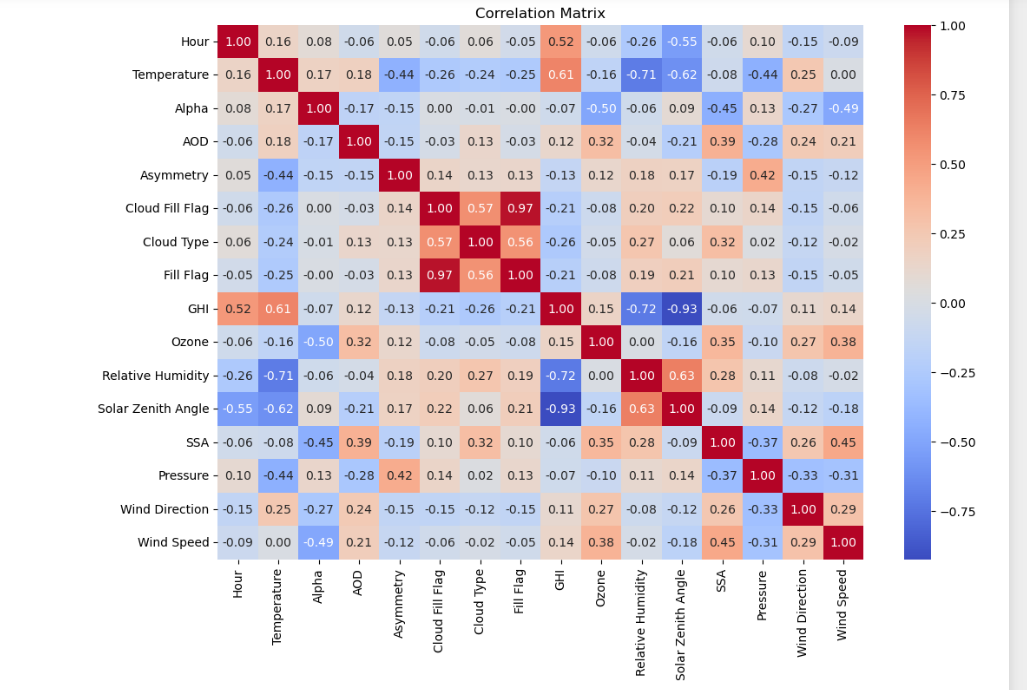
\includegraphics[width=1\linewidth]{fincorr.png}
            \caption{Final correlation matrix with reduced features.}
            \label{fig:enter-label}
        \end{figure}
         
    
    \label{Figure 1}




\subsection{Data Preprocessing}
Before initiating model training, the dataset/datasets were 
prepared to ensure its suitability for analysis. This would involve tasks such as cleaning the data to remove errors and inconsistencies. Using the insights from the feature seletcion step, it was determined that feature correlation values less than 0.07 were removed which resulted in 16 remaining features. Additionally, redundant features that exhibited high correlation with one another, such as the remaining solar radiation indicators (Clearsky GHI, Clearsky DHI, Clearsky DNI, DHI, DNI) and temporal indicators (year, month, day), were eliminated to avoid multicollinearity and improve model interpretability. Feature engineering was deemed unnecessary as the dat
aset already addressed missing values and provided clean, structured data for modeling. 
 
 


\subsection{Model training} The training process for the predictive models was designed to ensure robust evaluation and meaningful comparisons of their performance. The dataset was split into training and testing subsets, with 80 percent of the data allocated for training and 20 percent reserved for testing. This split was chosen to provide sufficient data for training the models while maintaining a substantial portion for independent evaluation.

\subsection{Hyperparameter Tuning}To optimize model performance, hyperparameters were explored through techniques such as grid search and  random search. This involved experimenting with different parameter combinations and evaluating their impact on model performance using cross-validation particularly for the decision tree regressor.



\subsection{Evaluation Metrics}

Model performance was evaluated using:
\begin{itemize}
    \item \textbf{Mean Absolute Error (MAE):} Measures the average magnitude of errors.
    \item \textbf{Root Mean Squared Error (RMSE):} Highlights the impact of large errors.
    \item \textbf{R-squared (R\textsuperscript{2}):} Indicates the proportion of variance explained by the model.
    \item \textbf{Predicted R\textsuperscript{2}:} Validated using cross-validation to ensure generalization.
\end{itemize}

A detailed comparison of these metrics across the three models quantifies their relative effectiveness in predicting GHI. For instance, while the linear regression model provides interpretability, its lower R\textsuperscript{2} score highlights the limitations of linear assumptions.
\section{Case Studies}

Using the presented methodology, the following case studies were explored:

\subsection{Case Study 1: Model Performance on San Francisco Dataset (2022)}
The first case study focused on evaluating the predictive performance of the models on the {San Francisco dataset for the year 2022}. Using the presented methodology, the optimal model of the three selected models was determined. 

\subsection{Case Study 2: Predicting San Francisco GHI Without Local Data using Combined Datasets of Nearby Locations}

In this case study, the objective was to explore how well the trained model from {San Mateo and Berkeley datasets} could predict \textbf{San Francisco's GHI} without direct access to its data. The datasets for San Mateo and Berkeley for the year of 2022, neighboring locations with similar climatic conditions to San Fransisco, were combined to train the model identified in Case Study 1 as the best model. 


\subsection{Case Study 3: Predicting San Francisco GHI Without Local Data using Combined Datasets of Farther Locations}

The third case study examined the predictive power of the Stacking Regressor when trained on the combiner datasets from Los Angeles and San Diego for the year of 2022, locations significantly farther from San Francisco with different climatic conditions.




\section{Results, Discussion, and Insights}
\subsection{Discussion and Analysis for Case Study 1}
For Case Study 1, the stacking regressor was observed to have achieved the highest accuracy, with an R\textsuperscript{2} score of 0.97, lowest Mean Absolute Error (MAE) of 27.4, and lowest Root Mean Squared Error (RMSE) of 48.9 outperforming individual models. Furthermore, a small difference between the actual R\textsuperscript{2} score of 0.973 and predicted R\textsuperscript{2} score of 0.966 demonstrate model robustness and the ability to generalize to new data.
The Decision Tree Regressor\ref{Figure 3} was seen to provide a strong standalone model for GHI prediction, offering interpretability and reliable performance, achieving performance metrics close to those of the Stacking Regressor. However, the slightly higher Mean Absolute Error (MAE) of 28.3 and Root Mean Squared Error (RMSE) of 51.0 and slightly lower  R\textsuperscript{2} value of 0.971, the scores suggest the Decision Tree slightly unperformed compared to the stacking regressor. Furthermore, this model may be more sensitive to specific patterns in the data. Its hierarchical structure made it particularly useful for understanding feature importance and nonlinear interactions. 
Linear regression\ref{Figure 2}, while interpretable, showed limitations in handling non-linear dependencies, achieving the highest MAE score of 57.38 and RMSE score of 80.49 and lowest R\textsuperscript{2} score of 0.93. 

Hence, it was observed that the linear regression's  limitations in handling nonlinear dependencies resulted in lower accuracy while the decision tree regressor's relatively small increase in error compared to the stacking regressor indicated that nonlinear features play a significant role in predicting GHI. Furthermore,
the stacking regressor was seen to leverage the complementary strengths of both models, reducing errors. These results demonstrate the effectiveness of ensemble methods in solar radiation prediction. Limitations include computational overhead and reliance on high-quality input data. Future work could explore deep learning techniques or incorporate real-time data for adaptive forecasting.
\subsection{Discussion and Analysis for Case Study 2} For Case Study 2, the objective was to predict Global Horizontal Irradiance (GHI) for San Francisco using a model trained on data from San Mateo and Berkeley, without direct access to San Francisco data. The stacking regressor using the data for just the combined dataset presented strong performance with low MAE and RMSE values of 15.42 and 37.01 and a high R\textsuperscript{2} value of 0.986.
The strong performance metrics reflect the geographic and climatic similarity between San Mateo and Berkeley, ensuring that the model could effectively learn from the shared patterns in solar radiation across the two locations. The results were then backtested on San Francisco dataset.
When the stacking regressor trained on the combined San Mateo and Berkeley dataset and  applied to the \{San Francisco dataset}, the results showed moderate success with MAE and RMSE values of 28.30 and 54.07 and a R\textsuperscript{2} of 0.967.  The moderate increase in MAE and RMSE suggests that while the San Mateo and Berkeley datasets provide a solid foundation for training, local nuances in San Francisco's solar radiation patterns could introduce additional complexity that the model struggles to capture. Despite these challenges, the \( R^2 \) score of 96.7\% indicates that the model generalizes reasonably well..
\subsection{Discussion and Analysis for Case Study 3}
For Case Study 3, the stacking regressor model trained on the combined datasets for Los Angeles and San Diego in the year 2022. This model demonstrated strong performance with low MAE and RMSE score of 17.95 and 43.38 and high R\textsuperscript{2} of 0.982. These performance metrics  indicate the ability of the stacking regressor to capture both linear and nonlinear dependencies in the Los Angeles and San Diego datasets, despite the geographic and climatic differences between these regions similar to San Mateo and Berkley. 
When the stacking regressor trained on the combined Los Angeles and San Diego dataset was applied to the San Francisco dataset, the results revealed challenges with higher MAE and RMSE score of 39.53 and 74.52 and lower R\textsuperscript{2} of 0.938. The significant increase in MAE and RMSE when applied to San Francisco underscores the challenges of using geographically distant training data. San Francisco's unique microclimates and atmospheric conditions, such as frequent fog, were not adequately represented in the Los Angeles and San Diego datasets.
\begin{figure}
            \centering
            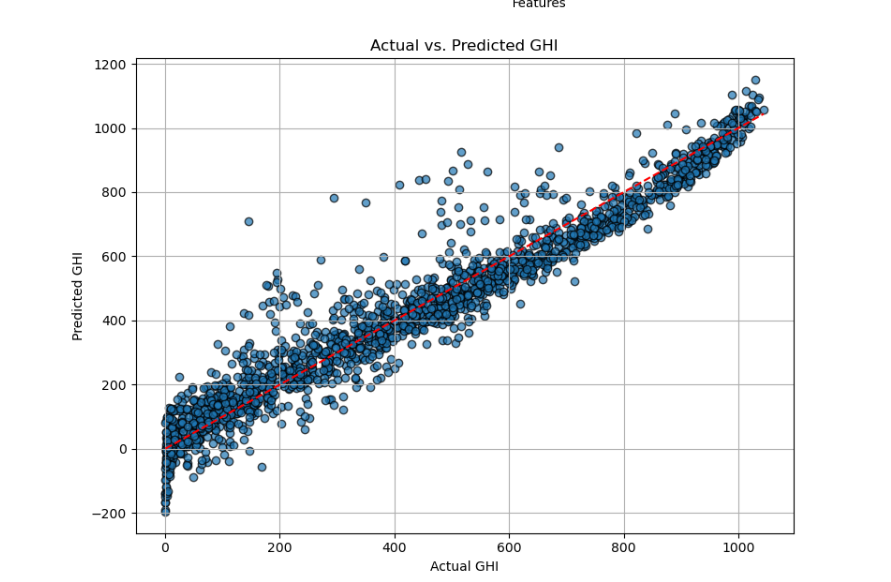
\includegraphics[width=1\linewidth]{ActualvsPredictedlinreg.png}
            \caption{Plot of actual vs predicted values for linear regression example.}
            \label{fig:enter-label}
        \end{figure}
         
    
    \label{Figure 2}
    \begin{figure}
            \centering
            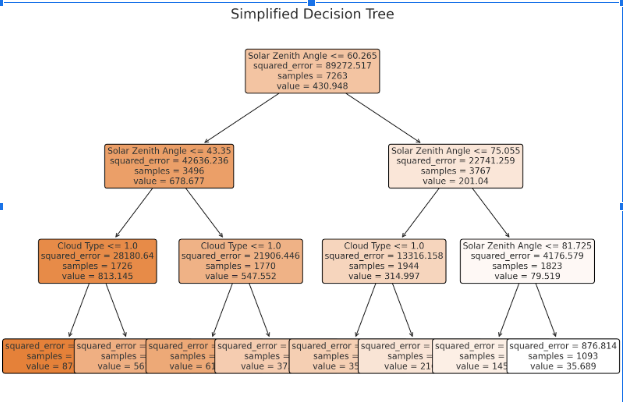
\includegraphics[width=1\linewidth]{Decisiontreevisualization.png}
            \caption{Visualization of Decision Tree.}
            \label{fig:enter-label}
        \end{figure}
         
    
    \label{Figure 3}



\subsubsection{Overall Discussion and Analysis}
 \paragraph{} Case Study 1 demonstrated the highest accuracy due to the availability of local data that captured specific climatic patterns. Next, Case Study 2 highlighted the potential of training on geographically similar regions, achieving moderate accuracy with minimal data loss. Finally, Case Study 3 revealed the most challenges, as difficulties of generalizing to San Francisco using data from distant locations were present, with higher errors and reduced robustness. Furthermore, The model's performance was strongly influenced by the geographic and climatic similarity of training data to the target location. Furthermore, neighboring regions (Case Study 2) provided sufficient overlap in climatic patterns, whereas distant regions (Case Study 3) introduced biases due to differences in solar radiation and atmospheric conditions. Additionaly, it  was observed that the stacking regressor effectively captured both linear and nonlinear dependencies, showing robustness across all cases. However, its reliance on high-quality, relevant input data limits its generalizability to regions with distinct microclimates or unique atmospheric patterns. Training on local or geographically similar data is crucial for accurate predictions, particularly for regions with unique weather phenomena. Furthermore, expanding datasets to include additional climatic variables or adaptive models could improve generalizability and reduce prediction errors.
  

\section{Ethical Considerations}

Data used in this project is sourced from publicly available repositories, ensuring compliance with ethical standards. However, the potential misuse of predictive models for unsustainable energy practices must be considered. One ethical concern lies in the potential biases introduced by the models due to limitations in the training data. For instance, in this project the data is primarily sourced from specific geographic regions, such as San Francisco, San Mateo, Berkeley, Los Angeles, and San Diego. Hence, this may not generalize well to locations with different climatic or atmospheric conditions. This could raises questions about the applicability and fairness of the models when deployed in underrepresented regions. Furthermore, the reliance on certain features, such as temperature and solar zenith angle, may overlook other factors critical to solar radiation in diverse settings, such as aerosol concentration or local pollution levels. Furthermore, the deployment of solar radiation prediction technology can have significant implications for addressing energy inequities. However, its implementation may inadvertently exacerbate existing inequalities. For isntance, regions with limited technological infrastructure or datasets may be excluded from the benefits of accurate solar radiation predictions, perpetuating global energy disparities. Additionally, advanced solar prediction models may disproportionately benefit wealthier regions with established renewable energy projects, sidelining communities with limited access to solar infrastructure. Ensuring diversity in both data collection and application is critical to the ethical use of these models. Collaboration with local communities to understand their unique solar energy needs and challenges can help adapt models for broader societal impact. Accurate solar radiation prediction models can contribute positively to sustainability and energy equity by enabling and improved predictions could help maximize solar energy production, reducing reliance on non-renewable energy sources. By supporting the expansion of renewable energy, these models could contribute to global efforts to reduce carbon emissions.
\section{Conclusion}

This project explored the development and evaluation of predictive models for solar radiation, specifically targeting Global Horizontal Irradiance (GHI). Through the use of linear regression, decision tree regression, and a stacking regressor, the study analyzed how different modeling techniques can address both linear and nonlinear dependencies in solar radiation data. The stacking regressor consistently demonstrated superior performance, highlighting the value of ensemble methods in capturing complex relationships.

The three case studies underscored the importance of data relevance and geographic similarity in model performance. Local data, as demonstrated in Case Study 1, provided the most accurate predictions, while models trained on geographically similar regions (Case Study 2) showed moderate success. However, the performance decline observed in Case Study 3, when trained on distant regions, emphasized the limitations of using non-local data.

Ethical considerations, including geographic bias, access to technology, and the societal implications of model deployment, were also addressed. These aspects highlight the necessity of equitable data practices, inclusive model design, and targeted deployment strategies to ensure that solar radiation prediction models contribute to global energy equity and sustainability.

The findings from this study reinforce the critical role of feature selection, robust model design, and diverse datasets in improving solar radiation predictions. Future work could expand on these insights by integrating deep learning techniques, real-time data inputs, and broader geographic representation. By addressing these areas, predictive models can become even more powerful tools for advancing renewable energy adoption and mitigating climate change.
\pagebreak
\newpage
\appendix

\newpage\section*{Appendix: Replication Instructions}

\subsection*{1. Software Requirements}
The following software and packages are required to replicate the project:
\begin{itemize}
    \item \textbf{Operating System:} The project is compatible with Windows, macOS, and Linux.
    \item \textbf{Python Version:} Python 3.8 or later.
    \item \textbf{Jupyter Notebook:} Install via Anaconda distribution or standalone.
    \item \textbf{Required Python Libraries:}
    \begin{itemize}
        \item pandas (version 1.3.3 or later)
        \item numpy (version 1.21.2 or later)
        \item scikit-learn (version 1.0.2 or later)
        \item matplotlib (version 3.4.3 or later)
        \item seaborn (version 0.11.2 or later)
    \end{itemize}
\end{itemize}

\subsection*{2. Installation Instructions}
\begin{enumerate}
    \item Install Python 3.8 or later from the official Python website (\url{https://www.python.org/}).
    \item Install Jupyter Notebook:
    \begin{verbatim}
    pip install notebook
    \end{verbatim}
    \item Install the required Python libraries:
    \begin{verbatim}
    pip install pandas numpy scikit-learn matplotlib seaborn
    \end{verbatim}
    \item Verify the installation by running the following command in the terminal or command prompt:
    \begin{verbatim}
    python -m pip list
    \end{verbatim}
    Ensure that the installed library versions match or exceed the required versions.
\end{enumerate}

\subsection*{3. Dataset Preparation}
\begin{itemize}
    \item The datasets used in this project include data from San Francisco, San Mateo, Berkeley, Los Angeles, and San Diego. Ensure you have access to these datasets in CSV format.
    \item Place all dataset files in a directory named \texttt{datasets} within the project folder.
    \item Ensure the datasets are preprocessed to align feature names and remove unnecessary columns as described in the methods section.
\end{itemize}

\subsection*{4. Running the Code}
\begin{enumerate}
    \item Launch Jupyter Notebook:
    \begin{verbatim}
    jupyter notebook
    \end{verbatim}
    \item Open the main project notebook file, \texttt{SolarRadiationPrediction.ipynb}.
    \item Run the notebook cells sequentially to execute the code. The notebook includes:
    \begin{itemize}
        \item Data preprocessing steps.
        \item Model training and evaluation.
        \item Visualizations and result analysis.
    \end{itemize}
    \item Outputs, including performance metrics and visualizations, will be generated in the notebook.
\end{enumerate}

\subsection*{5. Notes for Future Users}
\begin{itemize}
    \item \textbf{Compatibility:} Ensure compatibility of Python and library versions as updates may introduce breaking changes.
    \item \textbf{Reproducibility:} Use the provided requirements file to replicate the exact environment:
    \begin{verbatim}
    pip freeze > requirements.txt
    pip install -r requirements.txt
    \end{verbatim}
    \item \textbf{Dataset Updates:} If using newer datasets, ensure that they are preprocessed similarly to maintain consistency with the original analysis.
    \item \textbf{Error Handling:} Common errors, such as mismatched feature names, are documented in the notebook along with troubleshooting steps.
\end{itemize}

\subsection*{6. Additional Resources}
For further assistance, refer to the following resources:
\begin{itemize}
    \item Jupyter Notebook Documentation: \url{https://jupyter.org/}
    \item Python Package Index (PyPI): \url{https://pypi.org/}
    \item scikit-learn User Guide: \url{https://scikit-learn.org/stable/user_guide.html}
\end{itemize}

\newpage

\section*{Appendix: Code Architecture Overview}


\section*{Appendix: Code Architecture Overview}

This appendix provides an overview of the code architecture, outlining the structure and organization of the project. The goal is to enable another developer to extend, debug, or enhance the project effectively. The layout below reflects the structure of the Jupyter Notebook used in this project.

\subsection*{1. Project Structure}
The project is organized into the following directory and file structure:
\begin{verbatim}
project_root/
├── datasets/
│   ├── SanFrancisco.csv
│   ├── SanMateo.csv
│   ├── Berkeley.csv
│   ├── LosAngeles.csv
│   └── SanDiego.csv
├── notebooks/
│   └── SolarRadiationPrediction.ipynb
├── results/
│   └── output_visualizations/
├── requirements.txt
└── README.md
\end{verbatim}

\subsection*{2. Jupyter Notebook Cell Layout}
The Jupyter Notebook is organized into the following sections, with each section corresponding to specific cells:

\subsubsection*{1. Setup}
\begin{itemize}
    \item Import necessary libraries, including pandas, numpy, scikit-learn, matplotlib, and seaborn.
    \item Load required datasets and display their structure (e.g., using \texttt{head()}).
\end{itemize}

\subsubsection*{2. Data Preprocessing}
\begin{itemize}
    \item Clean datasets by removing unnecessary columns and handling missing values.
    \item Align feature names across all datasets to ensure consistency.
    \item Generate and visualize a correlation matrix to identify relationships between features and the target variable (GHI).
    \item Split data into training and testing sets with an 80/20 split.
\end{itemize}

\subsubsection*{3. Model Training}
\begin{itemize}
    \item Train and evaluate a Linear Regression model.
    \item Train and tune a Decision Tree Regressor, including hyperparameter tuning using GridSearchCV.
    \item Train a Stacking Regressor combining the Linear Regression and Decision Tree models.
\end{itemize}

\subsubsection*{4. Evaluation Metrics}
\begin{itemize}
    \item Compute performance metrics for each model:
    \begin{itemize}
        \item Mean Absolute Error (MAE).
        \item Root Mean Squared Error (RMSE).
        \item R-squared (\( R^2 \)).
        \item Predicted \( R^2 \) using cross-validation.
    \end{itemize}
    \item Display metrics in tabular form for comparison.
\end{itemize}

\subsubsection*{5. Visualization}
\begin{itemize}
    \item Generate scatter plots comparing actual vs. predicted GHI values for each model.
    \item Create residual plots to analyze prediction errors.
    \item Plot feature importance for the Decision Tree model.
    \item Visualize cross-validation scores for the Stacking Regressor.
\end{itemize}

\subsubsection*{6. Case Studies}
\begin{itemize}
    \item Analyze model performance on individual case studies, including:
    \begin{itemize}
        \item Localized predictions using San Francisco data.
        \item Predictions for San Francisco using models trained on combined San Mateo and Berkeley data.
        \item Predictions for San Francisco using models trained on combined Los Angeles and San Diego data.
    \end{itemize}
    \item Discuss insights and implications from each case study.
\end{itemize}

\subsubsection*{7. Conclusion}
\begin{itemize}
    \item Summarize findings from the models and case studies.
    \item Highlight strengths, limitations, and potential improvements.
\end{itemize}

\subsection*{3. Execution Workflow}
\begin{enumerate}
    \item Open the Jupyter Notebook \texttt{SolarRadiationPrediction.ipynb}.
    \item Execute cells sequentially, following the outlined structure.
    \item Save outputs, including performance metrics and visualizations, in the \texttt{results/} directory.
\end{enumerate}

\subsection*{4. Extensibility and Debugging}
\begin{itemize}
    \item \textbf{Adding New Features:} Developers can add new cells for additional preprocessing methods, models, or evaluation metrics.
    \item \textbf{Debugging:} Inline comments and logical grouping of cells make it easier to identify and fix issues.
    \item \textbf{Future Integration:} The notebook can be extended to include new datasets, advanced models, or deployment capabilities.
\end{itemize}

This layout ensures that the project is accessible for replication, extensibility, and debugging, enabling effective collaboration and adaptation.








\newpage
\begin{thebibliography}{200}

\bibitem{nsrdb} National Renewable Energy Laboratory. (n.d.). Retrieved from \url{https://nsrdb.nrel.gov/data-viewer}.

\bibitem{regression_models} Solar Power Prediction using Regression Models. Retrieved from \url{https://www.researchgate.net/publication/366613171_Solar_Power_Prediction_using_Regression_Models}.

\bibitem{iopscience} IOPscience. (n.d.-b). Retrieved from \url{https://iopscience.iop.org/article/10.1088/1755-1315/830/1/012080/pdf} and \url{https://www.azocleantech.com/article.aspx?ArticleID=1727}.

\bibitem{ensemble_models} Sehrawat, N., et al. (2023). Solar irradiance forecasting models using machine learning techniques and digital twin: A case study with comparison. Retrieved from \url{https://www.sciencedirect.com/science/article/pii/S2666603023000064}.

\bibitem{feature_selection} Gupta, R., Salcedo-Sanz, S., et al. (2024). Composition of feature selection techniques for improving the global horizontal irradiance estimation via machine learning models. Retrieved from \url{https://www.sciencedirect.com/science/article/abs/pii/S245190492400012X}.

\bibitem{ghi_topic} Global Horizontal Irradiance. (n.d.). Retrieved from \url{https://www.sciencedirect.com/topics/engineering/global-horizontal-irradiance}.

\bibitem{africa_hybrid_models} Kassem, Y., Camur, H., Adamu, M. T., Chikowero, T., & Apreala, T. Prediction of solar irradiation in Africa using linear-nonlinear hybrid models. Retrieved from \url{https://www.etasr.com/index.php/ETASR/article/view/6131}.

\bibitem{site_adaptation} Narvaez, G., Giraldo, L. F., Bressan, M., & Pantoja, A. (2023). Machine learning for site-adaptation and Solar Radiation Forecasting. Retrieved from \url{https://hal.science/hal-04070113}.

\bibitem{geospatial_ethics} Geospatial Data. Ethics & Applications of Geospatial Technologies. LibGuides at University of Texas at Austin. Retrieved from \url{https://guides.lib.utexas.edu/grg356t}. Accessed 22 Apr. 2024.

\bibitem{geodata_privacy} Privacy Challenges in Geodata and Open Data. Retrieved from \url{https://rgs-ibg.onlinelibrary.wiley.com/doi/full/10.1111/area.12888}. Accessed 22 Apr. 2024.

\bibitem{thin_films} Nkuissi, H. J. T., Konan, F. K., Hartiti, B., & Ndjaka, J.-M. (2020). Toxic materials used in thin film photovoltaics and their impacts on environment. Retrieved from \url{https://www.intechopen.com/chapters/68288}.

\bibitem{toxic_solar} Shellenberger, M. (2022). Dark Side to Solar? More Reports Tie Panel Production to Toxic Pollution. Forbes. Retrieved from \url{https://www.forbes.com/sites/michaelshellenberger/2021/06/21/why-everything-they-said-about-solar---including-that-its-clean-and-cheap---was-wrong/?sh=7f50ab595fe5}.

\bibitem{human_rights_solar} Solar vs Human Rights: Hidden Ethical Issues with Solar Panels. (n.d.). Retrieved from \url{https://www.frdm.co/blogs/solar-vs-human-rights}.

\bibitem{energy_proceedings} Energy Proceedings. (n.d.). Machine learning models for solar irradiance prediction. Retrieved from \url{https://www.energy-proceedings.org/wp-content/uploads/icae2021/1642315686.pdf}.

\end{thebibliography}





\printbibliography
\end{document}



